\chapter{xv6实验系统实例分析——从命令cat讲起}

在假设目录下有test.txt文件(准备阶段完成)的前提下,我们将要分析执行以下命令的过程中,xv6所做的工作。

\shell{cat test.txt}

\section{准备阶段}

\subsection{文件准备}

执行命令前,我们先使用下列命令在默认目录(xv6进入后的目录)新建了test.txt文件,并往里写入了内容“test”。

\shell{echo test > test.txt}

\subsection{xv6当前的文件}

\begin{figure}[H]
  \centering
  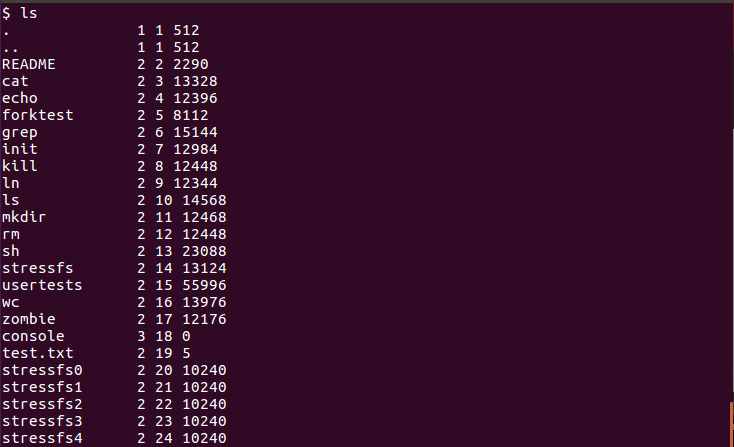
\includegraphics[width=6in]{figures/eg/files.png}
  \caption{xv6当前目录内容}
\end{figure}

\section{开始阶段}

\subsection{用户输入命令过程}

我们要在键盘上输入 cat test.txt \\n 这些字符,在输入这些字符的过程之中,每输入一个字符,键盘通过usb数据线向cpu发出了中断请求,cpu会转去执行中断服务程序,我们的中断服务程序是由xv6系统定义的.

trap.c这个文件包含了xv6对不同的中断的处理过程以及中断表的初始化。

Tvinit函数主要完成对idt表进行初始化。其中vectors中存放的是每个中断处理程序的入口地址。vectors的定义是在vectors.S中, 由一个perl程序vectors.pl生成。另外对tickslock这个锁进行初始化,这个锁是用来处理时钟中断的。

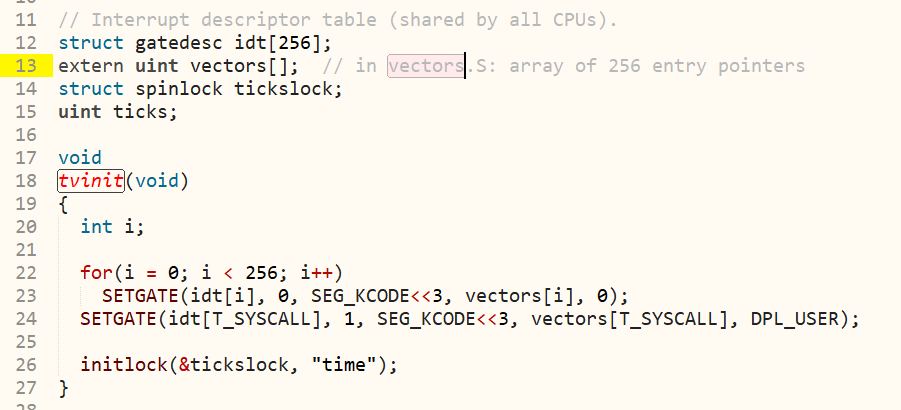
\includegraphics[width=6in]{figures/input/image1.png}

idtinit是用来加载idt表的。idtinit之所以和tvinit分开的原因是xv6支持多核心,所以idtinit会被多个CPU调用。但是tvinit过程只需要被调用一次。

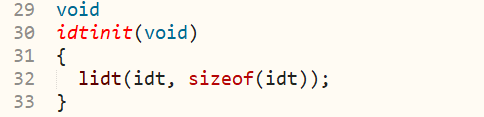
\includegraphics[width=6in]{figures/input/image2.png}

对应的中断处理过程是在trap函数之中.所有的中断在经过中断入口程序(trapasm.S中定义)后,都会最终跳转到这里。其处理过程如下:

  \begin{enumerate}
  \item 在39~47行,判断中断是系统调用,若是则通过syscall过程完成系统调用的处理。值得注意的是,这里进行了当前进程是否被其他进程kill的情况。也就是说,如果一个进程被其他进程Kill,那么此进程将在进入或退出内核态时被切断。
  \item 49~95行是对不同的中断进行处理。
  \item 第50行case IRQ\_OFFSET+IRQ\_TIMER是处理时钟中断,如果当前CPU是0号CPU,那么ticks将增加一,同时进行对处于sleeping状态的进程进行检查(通过wakeup)。在wakeup中,一旦发现某些进程休眠的时间结束,则把其转化成RUNNABLE;
  \item 59~62行通过 ideintr()完成磁盘中断处理;
  \item 66~69行通过kbdintr()完成键盘中断处理;
  \end{enumerate}

  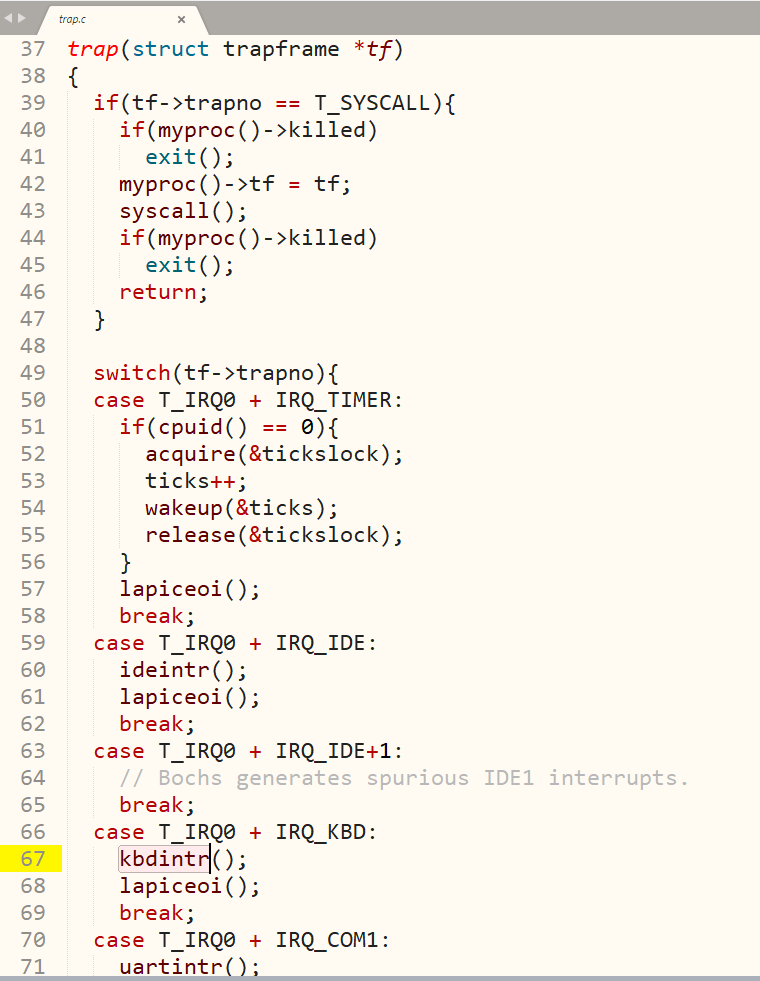
\includegraphics[width=6in]{figures/input/image3.png}

  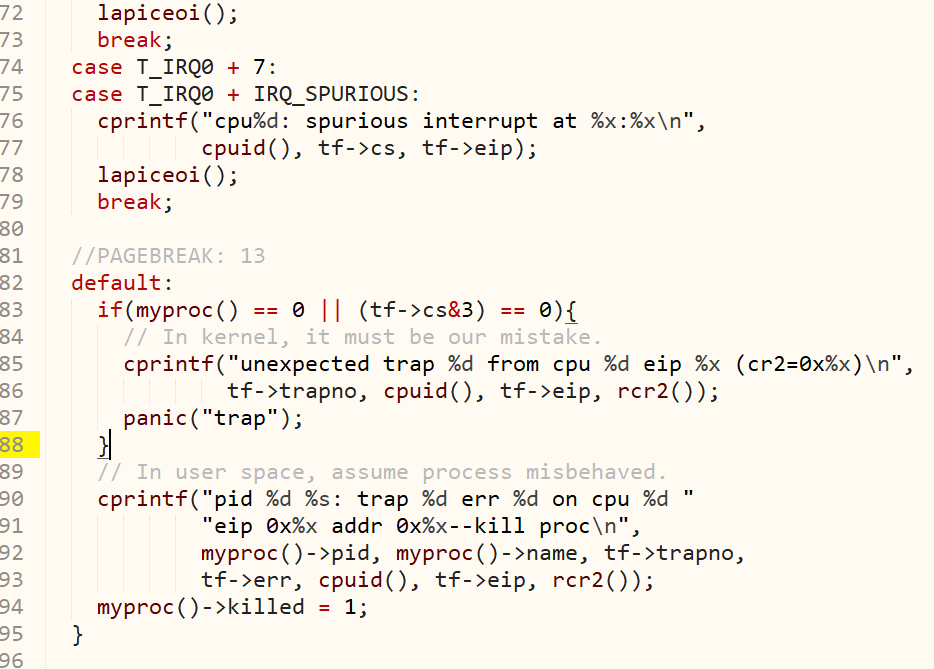
\includegraphics[width=6in]{figures/input/image4.png}

而中断向量的入口地址和入口程序是由vectors.S来定义的.( vectors.S是由vectors.pl生成的)可以注意到,中断分成两类:一类是压入错误编码的(error code), 另一类不会压入错误编码。因此对于第二类,vectors.S将压入一个0。此外vectors.S还会将中断号压入栈。在压完两个必要的值之后,所有中断都将统一的跳转进入alltraps入口程序。

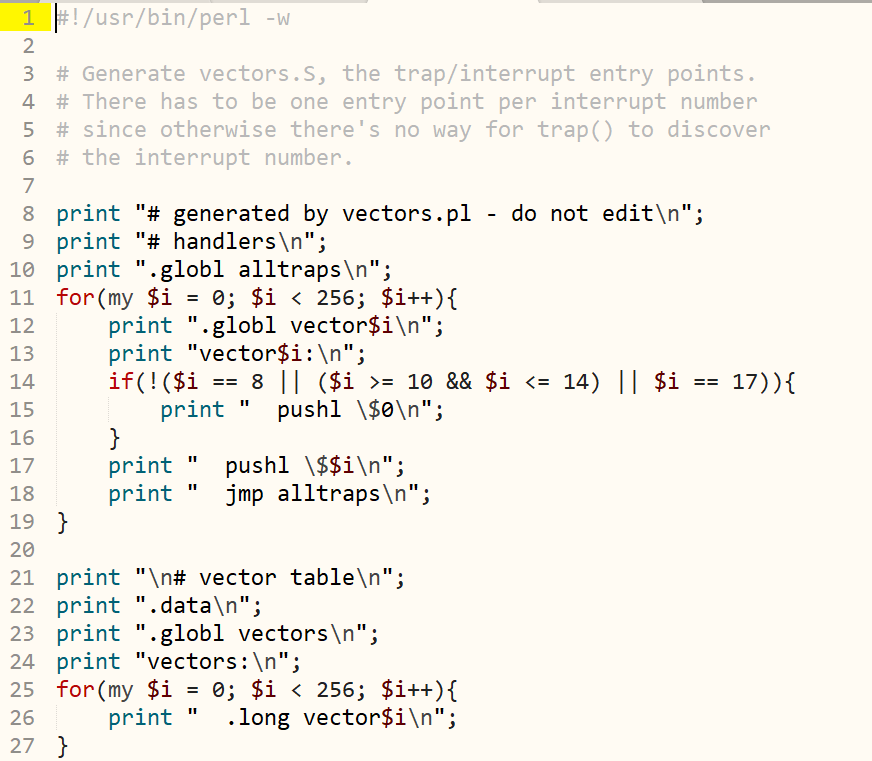
\includegraphics[width=6in]{figures/input/image5.png}

Cpu在检测到键盘的中断请求之后,如果允许中断的话,就转去执行中断服务程序,而中断向量号在traps.h之中就已经定义好了.

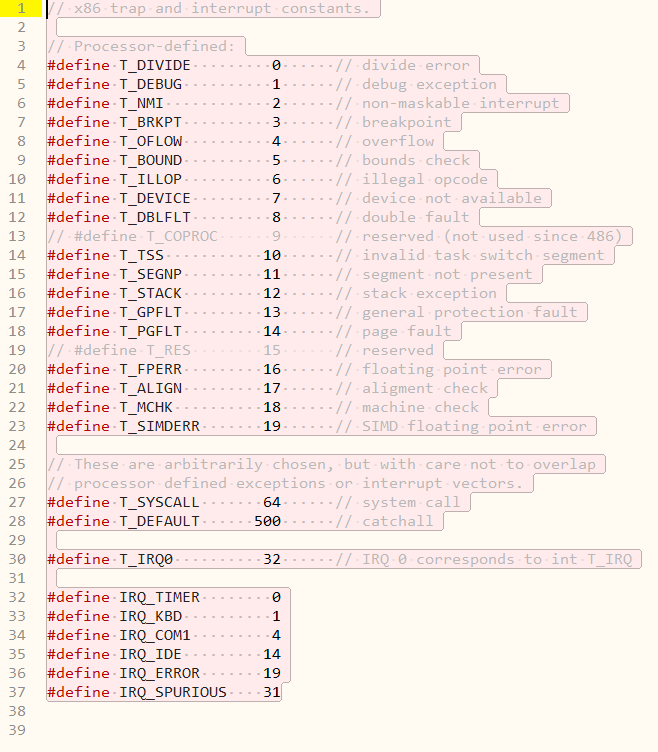
\includegraphics[width=6in]{figures/input/image6.png}

由于xv6在启动过程之中已经完成了中断表的初始化,现在由于键盘事件产生了中断请求, 在vectors.S之中,将在栈内压入一个0,键盘事件的中断号然后就会跳转到alltraps.完成一些保存寄存器的操作,然后在14~16行是将段寄存器换到内核段。然后调用trap.c中的trap函数。因为trap的参数是指向trapframe的指针,所以将esp寄存器压入栈,其正好是trapframe的地址。

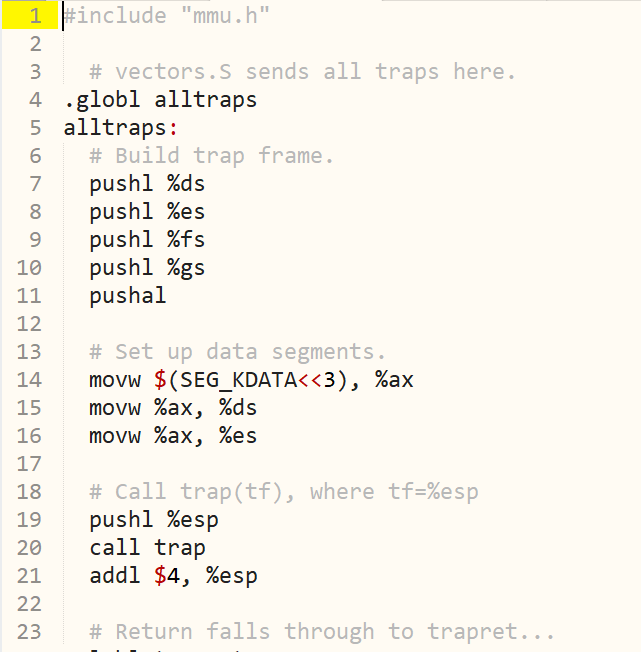
\includegraphics[width=6in]{figures/input/image7.png}

由于之前栈你已经有了中断向量号,trap就会去执行中断服务程序kbdintr,而这个函数是定义在kdb.c函数之中,

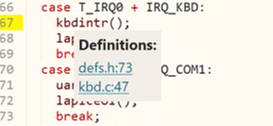
\includegraphics[width=6in]{figures/input/image8.png}

转到对应的位置,发现kbdintr的定义如下图所示, kbdintr调用了consoleintr函数

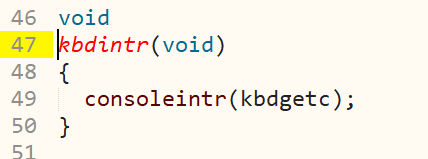
\includegraphics[width=6in]{figures/input/image9.png}

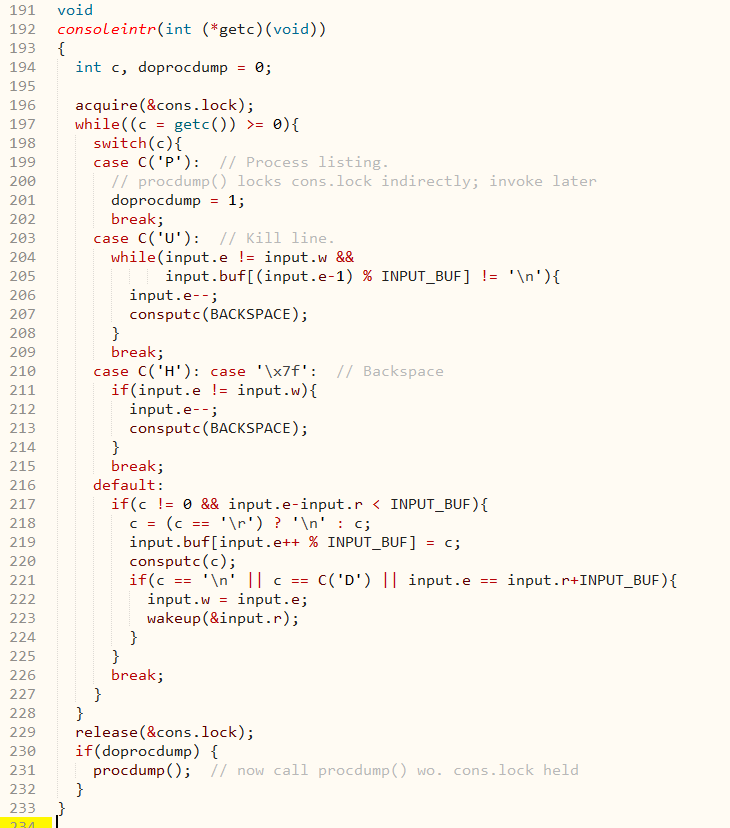
\includegraphics[width=6in]{figures/input/image10.png}


通过分析consoleintr 函数我们可以得知, consoleintr 函数会根据参数getc获取用户的输入,根据用户的输入做出不同的响应, consoleintr在处理很多字符的时候会调用 consputc 函数


\includegraphics[width=6in]{figures/input/image11.png}

然后consputc函数会调用 cgaputs 函数来将数据输出到显示器之上.


\includegraphics[width=6in]{figures/input/image12.png}

在执行完中断处理函数之后,返回到我们的os中,继续执行我们的代码.


\subsection{创建cat进程}

创建cat进程可分为3个步骤:

\begin{enumerate}
\item shell用fork1函数拷贝了一个子进程
\item shell子进程调用runcmd执行cat进程
\item shell父进程等待子进程结束
\end{enumerate}

代码如下:

\begin{minted}{C}
if(fork1() == 0)
  runcmd(parsecmd(buf));
wait();
\end{minted}

\subsubsection{拷贝子进程}

拷贝子进程需要以下几步:

\begin{enumerate}
\item 父进程使用上面实现的set\_pgfault\_handler()设置pgfault()为页错误处理程序
\item 父进程调用 sys\_exofork() 来建立子进程。
\item 对于父进程的每一个可写的页或者写入时复制的页,父进程会调用 duppage(),来让页面映射到子进程的地址空间中并且重新映射该页面到自己的地址空间中。
\item 父进程为子进程设置用户页错误的入口(跟自己的一样)。
\item 子进程可以运行(enable)。
\end{enumerate}

fork1代码如下:

\begin{minted}{C}
int
fork1(void)
{
  int pid;

  pid = fork();
  if(pid == -1)
    panic("fork");
  return pid;
}
\end{minted}

可以看出,fork1()仅仅是添加了错误判断的fork()函数。

我们继续看fork:

首先,先获取当前的进程(父进程)信息:

\begin{minted}{C}
  struct proc *curproc = myproc();
\end{minted}

然后,申请一个新的未使用的进程:

\begin{minted}{C}
np = allocproc()
\end{minted}

我们先深入一下allproc()函数。

\begin{minted}{C}
  for(p = ptable.proc; p < &ptable.proc[NPROC]; p++)
    if(p->state == UNUSED)
      goto found;
\end{minted}

我们发现,在param.h中,NPROC被定义为64(\mintinline{C}{#define NPROC        64  // maximum number of processes})。因此,xv6最多支持64个进程。

在allproc()中,遍历所有的进程表,找到一个没有在用的(UNUSED),然后就可以进行进一步的处理,并返回该进程信息。

首先需要修改状态、获取新的pid:

\begin{minted}{C}
  p->state = EMBRYO;
  p->pid = nextpid++;
\end{minted}

然后调用kalloc()申请系统栈空间:

\begin{minted}{C}
  if((p->kstack = kalloc()) == 0){
    p->state = UNUSED;
    return 0;
  }
\end{minted}

接着申请内存为上下文信息TrapFrame申请内存:

\begin{minted}{C}
  // Leave room for trap frame.
  sp -= sizeof *p->tf;
  p->tf = (struct trapframe*)sp;
\end{minted}

最后设置上下文信息:

\begin{minted}{C}
  // Set up new context to start executing at forkret,
  // which returns to trapret.
  sp -= 4;
  *(uint*)sp = (uint)trapret;

  sp -= sizeof *p->context;
  p->context = (struct context*)sp;
  memset(p->context, 0, sizeof *p->context);
  p->context->eip = (uint)forkret;
\end{minted}

回到fork()函数,接下来就需要父进程信息拷贝到子进程。

首先,由于xv6使用的是fork时惰性地复制页表,而页表指向的页只有在修改时才会进行复制(就是写时复制),因此只需要调用copyuvm()将页表复制一份,并将涉及到的writable和写时复制的页都设置成写时复制。新页表给子进程用:

\begin{minted}{C}
  if((np->pgdir = copyuvm(curproc->pgdir, curproc->sz)) == 0){
    kfree(np->kstack);
    np->kstack = 0;
    np->state = UNUSED;
    return -1;
  }
\end{minted}

然后设置一下子进程的大小,祖先信息和寄存器信息等等:

\begin{minted}{C}
  np->sz = curproc->sz;
  np->parent = curproc;
  *np->tf = *curproc->tf;
  // Clear %eax so that fork returns 0 in the child.
  np->tf->eax = 0;
  pid = np->pid;
\end{minted}

最后,获取ptable.lock,设置子进程可以运行(enable),然后释放ptable.lock。

\begin{minted}{C}
  acquire(&ptable.lock);
  np->state = RUNNABLE;
  release(&ptable.lock);
\end{minted}

\subsubsection{执行cat程序}

向parsecmd()函数传入命令,就可以得到cmd结构体,在此例中返回的是execcmd结构体。

\begin{minted}{C}
struct execcmd {
  int type;
  char *argv[MAXARGS];
  char *eargv[MAXARGS];
};
\end{minted}

然后该结构体传入runcmd()函数,由于cat text.txt命令没有其他复杂的内容(例如管道,重定向等等),因此进入到runcmd()函数之后,被分类为EXEC。另外几种还有:REDIR,LIST,PIPE,BACK。

观察代码:

\begin{minted}{C}
case EXEC:
  ecmd = (struct execcmd*)cmd;
  if(ecmd->argv[0] == 0)
    exit();
  exec(ecmd->argv[0], ecmd->argv);
  printf(2, "exec %s failed\n", ecmd->argv[0]);
  break;
\end{minted}

最后会执行exec()执行cat,覆盖当前shell子进程。我们继续跟踪exec()。

exec()函数(\mintinline{C}{int exec(char *path, char **argv)})在exec.c中。

首先,需要用namei获取path路径的文件对应的的inode。

\textbf{注}:文件操作内容请看后面cat读取文件过程的讲解。

然后检查ELF文件头(由于xv6仅支持ELF文件,所以需要对文件有效性做一些验证):

\begin{minted}{C}
  // Check ELF header
  if(readi(ip, (char*)&elf, 0, sizeof(elf)) != sizeof(elf))
    goto bad;
  if(elf.magic != ELF_MAGIC)
    goto bad;
\end{minted}

接下来,需要设置内核态虚拟内存,然后根据ELF头中存储的信息为每个程序段申请内存。对于每个程序段,加载对应内容存入内存。

\begin{minted}{C}
  // Load program into memory.
  sz = 0;
  for(i=0, off=elf.phoff; i<elf.phnum; i++, off+=sizeof(ph)){
    if(readi(ip, (char*)&ph, off, sizeof(ph)) != sizeof(ph))
      goto bad;
    if(ph.type != ELF_PROG_LOAD)
      continue;
    if(ph.memsz < ph.filesz)
      goto bad;
    if(ph.vaddr + ph.memsz < ph.vaddr)
      goto bad;
    if((sz = allocuvm(pgdir, sz, ph.vaddr + ph.memsz)) == 0)
      goto bad;
    if(ph.vaddr % PGSIZE != 0)
      goto bad;
    if(loaduvm(pgdir, (char*)ph.vaddr, ip, ph.off, ph.filesz) < 0)
      goto bad;
  }
\end{minted}

接下来需要设置用户栈。xv6用了一种巧妙的方法,即可以节约初始时用户栈所需的内存,也可以避免访问越界造成的问题。方法就是:设置两个页为用户栈,然后一个用作用户栈,一个设置成inaccessible,这样就可以两者兼顾,非常巧妙。

\begin{minted}{C}
  // Allocate two pages at the next page boundary.
  // Make the first inaccessible.  Use the second as the user stack.
  sz = PGROUNDUP(sz);
  if((sz = allocuvm(pgdir, sz, sz + 2*PGSIZE)) == 0)
    goto bad;
  clearpteu(pgdir, (char*)(sz - 2*PGSIZE));
  sp = sz;
\end{minted}

接下来把所有参数压到栈中。

\begin{minted}{C}
  // Push argument strings, prepare rest of stack in ustack.
  for(argc = 0; argv[argc]; argc++) {
    if(argc >= MAXARG)
      goto bad;
    sp = (sp - (strlen(argv[argc]) + 1)) & ~3;
    if(copyout(pgdir, sp, argv[argc], strlen(argv[argc]) + 1) < 0)
      goto bad;
    ustack[3+argc] = sp;
  }
  ustack[3+argc] = 0;
  ustack[0] = 0xffffffff;  // fake return PC
  ustack[1] = argc;
  ustack[2] = sp - (argc+1)*4;  // argv pointer
  sp -= (3+argc+1) * 4;
\end{minted}

接下来设置进程的上下文环境:

\begin{minted}{C}
  // Commit to the user image.
  oldpgdir = curproc->pgdir;
  curproc->pgdir = pgdir;
  curproc->sz = sz;
  curproc->tf->eip = elf.entry;  // main
  curproc->tf->esp = sp;
  switchuvm(curproc);
  freevm(oldpgdir);
  return 0;
\end{minted}

这样,CPU在下次调度时,就可能会执行cat这个进程。

\section{执行阶段}

\subsection{准备工作}

cat程序的代码非常简单:

\begin{minted}{C}
#include "types.h"
#include "stat.h"
#include "user.h"

char buf[512];

void
cat(int fd)
{
  int n;

  while((n = read(fd, buf, sizeof(buf))) > 0) {
    if (write(1, buf, n) != n) {
      printf(1, "cat: write error\n");
      exit();
    }
  }
  if(n < 0){
    printf(1, "cat: read error\n");
    exit();
  }
}

int
main(int argc, char *argv[])
{
  int fd, i;

  if(argc <= 1){
    cat(0);
    exit();
  }

  for(i = 1; i < argc; i++){
    if((fd = open(argv[i], 0)) < 0){
      printf(1, "cat: cannot open %s\n", argv[i]);
      exit();
    }
    cat(fd);
    close(fd);
  }
  exit();
}
\end{minted}

29-32行中,尝试从参数列表中获取参数,如果$argc \leq 1$,说明cat命令后没有加参数,此时无法正常执行程序。否则则可以继续执行。

34-41行执行的任务是:将所有文件打开,然后调用cat函数,然后关闭所有文件。在此过程中,cat会尝试对每一个参数中代表的文件名尝试进行打开,如果打开不了,就会提示无法打开,并调用exit()退出程序。

执行结束后,42行调用exit(),程序执行结束。

\subsection{读入文件}

Cat程序需要将它要输出的文件加载到缓冲区,再从缓冲区写到输出流,这个输出流可以是控制台也可以是文件。

首先打开文件

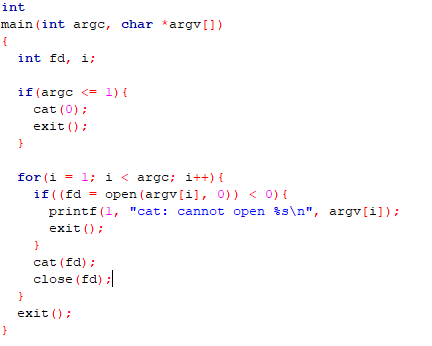
\includegraphics[width=6in]{figures/eg_file/image168.png}

使用文件系统提供的统一接口open打开文件,得到一个文件描述符fd。Xv6中的文件操作是以系统调用形式提供的。Open就是一个系统调用,调用sys\_open函数,类似的还有read,write,close等函数。
Sys\_open函数如下

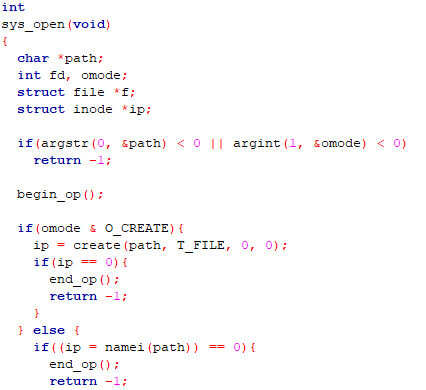
\includegraphics[width=6in]{figures/eg_file/image169.png}

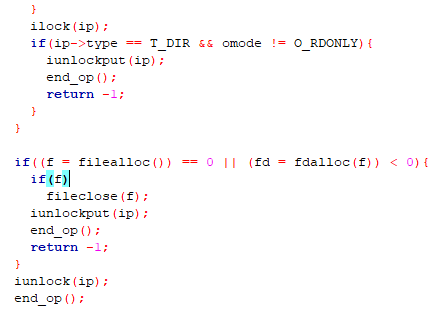
\includegraphics[width=6in]{figures/eg_file/image170.png}

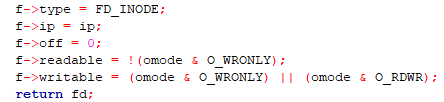
\includegraphics[width=6in]{figures/eg_file/image171.png}



在打开文件时,open函数会使用文件路径来调用namei打开文件返回inode节点指针。接着为了保证多进程安全,实现一个inode节点只能被一个进程操作,调用ilock将inode节点锁住。调用ilock加锁的另外一个原因是它会将inode的信息(如下面的ip->type)加载到内存中。
获得inode指针后,系统开始调用filealloc申请新的文件描述符,然后将文件信息和inode指针打包起来返回给上一层。这样cat函数就得到了需要打开的文件的文件描述符fd。Cat函数可以使用这个fd进行读写操作。
在分析cat函数下一步之前我们观察一下namei函数。

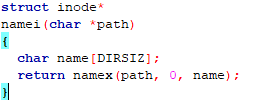
\includegraphics[width=6in]{figures/eg_file/image172.png}


Namei函数承担的是寻找并打开文件的功能,输入路径返回inode指针和文件名,它是对namex函数的加上文件名的又一层包装。Namex函数负责使用路径查找inode。

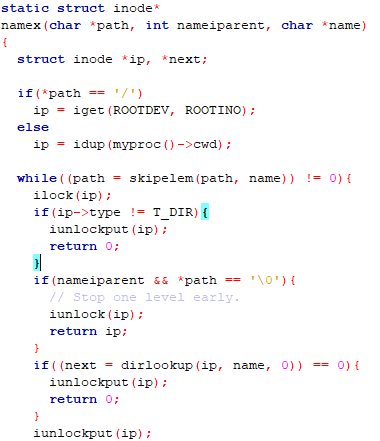
\includegraphics[width=6in]{figures/eg_file/image173.png}

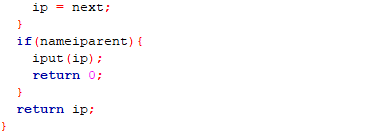
\includegraphics[width=6in]{figures/eg_file/image174.png}

如果地址以/开头那么从根目录开始找,否则从当前目录开始找。一层一层通过dirlookup函数匹配目录名,对每层目录调用dirlookup寻找下一层目录节点。直到找到目标文件或者找不到跳出。这个过程与jos中的walk\_path相近。
接下来我们回到cat函数,分析系统是怎么将文本从文件中读出来,又写到控制台中去的。

Cat函数的核心代码

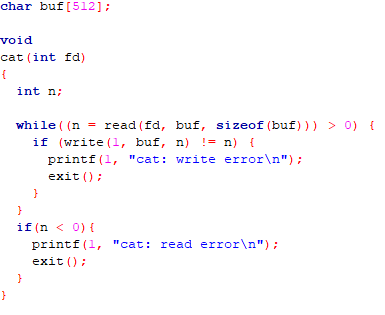
\includegraphics[width=6in]{figures/eg_file/image175.png}


函数使用一个大小512的buf做中转,每次从fd
文件里用read函数读取一个buf,再用write写到控制台或者文件或者其他输出流。
前文说过read和write都是系统调用。本体在sys\_read和sys\_write。观察sys\_read。

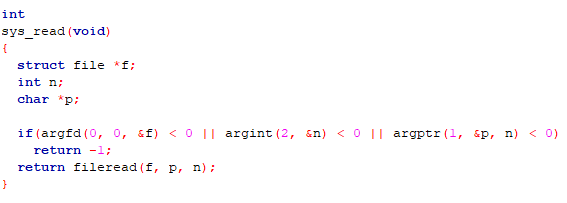
\includegraphics[width=6in]{figures/eg_file/image176.png}

Sys\_read做了简单检查,将参数传给fileread函数。

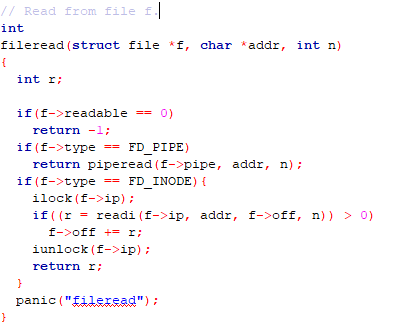
\includegraphics[width=6in]{figures/eg_file/image177.png}

Fileread函数判断出来是读文件也就是inode的时候,他会将文件inode锁上,然后调用readi函数。

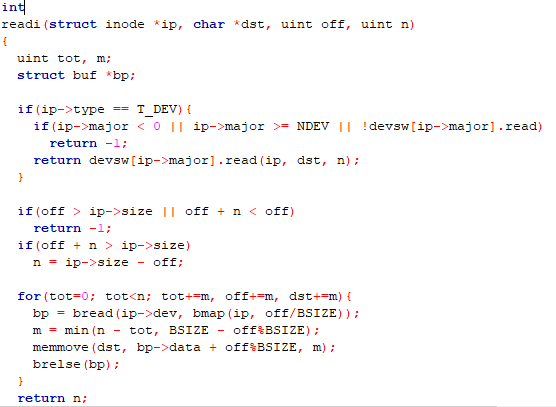
\includegraphics[width=6in]{figures/eg_file/image178.png}

Readi函数真正执行了读文件的操作。循环使用bread函数,将文件一块一块搬到缓冲区中实现读文件。

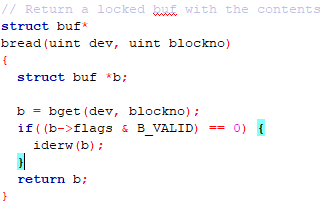
\includegraphics[width=6in]{figures/eg_file/image179.png}

Bread函数中使用bget(dev,blockno)来调用文件对应的磁盘设备来读取响应的块。这里的dev是底层文件系统实现对磁盘驱动做的统一封装成的设备。

最后再这么一层层将buf返回上去,我们就完成了一次读文件操作。接下来就应该调用write的系统调用来将读完的buf写到控制台了。

\subsection{输出结果}


write和read对称,结构基本类似。这里我们要将文本输出到控制台,而控制台的文件描述符为1,于是我们调用write(1, buf, n)。sys\_write类似的调用filewrite,再调用writei。

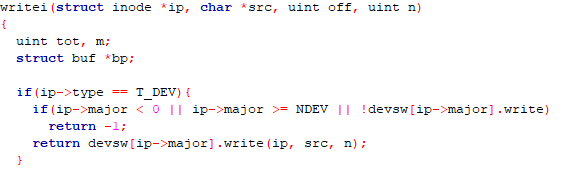
\includegraphics[width=6in]{figures/eg_file/image180.png}

此时应当输出到控制台这个“设备”中。底层文件系统已经帮我们将磁盘,屏幕,控制台等各种设备都抽象成了“设备”,于是控制台的设备读写函数将帮助我们输出到控制台,也就是console。Console对应的写函数为consolewrite。

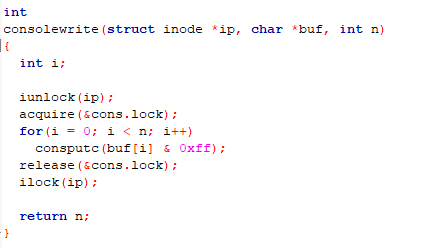
\includegraphics[width=6in]{figures/eg_file/image181.png}

Consolewrite一开始先将文件inode锁上以防并发写操作而出错。紧接着将控制台锁上以防输出混乱。接下来就可以调用consputsc将buf中的字符一个一个推到控制台中,进而显示在屏幕上了。



\subsection{中间过程:程序调度}

在cat运行过程中,如果其主动放弃其时间片,CPU会对其进行调度。CPU调度所有进程的方式如下:

当CPU启动之后,执行scheduler函数。scheduler函数内部有一个无限循环,每次循环为一个周期。在每个周期里,从进程表中找到一个RUNNABLE的进程,切换为进程的上下文,此时开始执行函数。当函数运行结束时,调用return函数,此时切换为CPU的上下文,开始下一循环。

初始化部分:在schedulre()函数中,首先调用mycpu()获取当前CPU信息,然后将该CPU的当前正在运行的进程设为0,表示无进程在运行:

\begin{minted}{C}
  struct cpu *c = mycpu();
  c->proc = 0;
\end{minted}

调度部分:遍历进程表,检查是否有进程为RUNNABLE状态(可以运行但未在运行)。如果有,就将CPU的当前运行进程设为该进程,然后用switchuvm()修改CPU的GDT等信息。之后使用swtch()函数切换进程(修改上下文环境),最后修改内核虚拟地址空间。

\begin{minted}{C}
    for(p = ptable.proc; p < &ptable.proc[NPROC]; p++){
      if(p->state != RUNNABLE)
        continue;

      // Switch to chosen process.  It is the process's job
      // to release ptable.lock and then reacquire it
      // before jumping back to us.
      c->proc = p;
      switchuvm(p);
      p->state = RUNNING;

      swtch(&(c->scheduler), p->context);
      switchkvm();

      // Process is done running for now.
      // It should have changed its p->state before coming back.
      c->proc = 0;
    }
\end{minted}

\subsection{中间过程:休眠唤醒}

xv6中有多种IRQ,有IRQ\_TIMER、IRQ\_IDE、IRQ\_KBD等等。其中IRQ\_TIMER指的是时钟中断,当时钟终端到来时,会调用wakeup()函数。我们看一下trap.c中的trap函数的片段:

\begin{minted}{C}
  switch(tf->trapno){
  case T_IRQ0 + IRQ_TIMER:
    if(cpuid() == 0){
      acquire(&tickslock);
      ticks++;
      wakeup(&ticks);
      release(&tickslock);
    }
    lapiceoi();
    break;
\end{minted}

wakeup()函数会调用wakeup1()函数。wakeup1()函数会遍历所有的进程,然后找到SLEEPING的进程,然后设为RUNNABLE。wakeup1()函数的内容如下:

\begin{minted}{C}
//PAGEBREAK!
// Wake up all processes sleeping on chan.
// The ptable lock must be held.
static void
wakeup1(void *chan)
{
  struct proc *p;

  for(p = ptable.proc; p < &ptable.proc[NPROC]; p++)
    if(p->state == SLEEPING && p->chan == chan)
      p->state = RUNNABLE;
}
\end{minted}


\section{结束阶段}

在程序结束阶段,会调用exit()函数。

exit()函数在proc.c中。主要步骤如下:

首先遍历文件表。文件表大小最大为NOFILE=16个,也就是说一个进程最多打开16个文件。遍历文件表时,查看是否打开过该文件,如果打开过就调用fileclose()函数来关闭文件占用。

\begin{minted}{C}
  // Close all open files.
  for(fd = 0; fd < NOFILE; fd++){
    if(curproc->ofile[fd]){
      fileclose(curproc->ofile[fd]);
      curproc->ofile[fd] = 0;
    }
  }
\end{minted}

之后唤醒当前进程的父进程,因为有可能父进程调用了wait()函数,在等待子进程结束返回。

\begin{minted}{C}
  // Parent might be sleeping in wait().
  wakeup1(curproc->parent);
\end{minted}

最后,把进程设成ZOMBIE状态(僵死程序,随时可以清理),调用sched()函数手动进程进程调度。

\begin{minted}{C}
  // Jump into the scheduler, never to return.
  curproc->state = ZOMBIE;
  sched();
\end{minted}
